\documentclass[conference]{IEEEtran}
\IEEEoverridecommandlockouts
\usepackage{cite}
\usepackage{amsmath,amssymb}
\usepackage{graphicx}
\usepackage{booktabs}
\usepackage{xcolor}
\usepackage{url}

% Headline numbers used in the running text. Every value is copied from
% research_brief.md (section given in the comment). Tables in main.tex hold
% the rest. To update after new runs, change the value here only.

% Setup
\newcommand{\nSeeds}{10}
\newcommand{\nRows}{10{,}000}
\newcommand{\nEpochs}{150}
\newcommand{\realTSTR}{0.856}            % Setup: real-data TSTR baseline

% Damage, 10 seeds (F, "Damage, 10 seeds"): last-check test TSTR, mean of 10 samples
\newcommand{\dmgCtrl}{0.804}
\newcommand{\dmgThree}{0.777}
\newcommand{\dmgTen}{0.766}
\newcommand{\dmgThirty}{0.748}
\newcommand{\dmgHundred}{0.732}

% Past-only detection, aggregate score, expanding reference, h = 5 (F)
\newcommand{\scoreExpDet}{39}            % of 40 spiked runs
\newcommand{\scoreExpCtrl}{0}            % of 10 controls
\newcommand{\tstrDet}{13}                % TSTR mean of 10, expanding, of 40

% Roll back and continue (H), last check, mean of 10 seeds
\newcommand{\rbLow}{0.803}
\newcommand{\rbHigh}{0.805}

% From-the-start learning rate x10 (I)
\newcommand{\highlrCost}{4.2}            % accuracy points, last check

% TSTR noise (B)
\newcommand{\tstrSampleSdLow}{0.016}
\newcommand{\tstrSampleSdHigh}{0.018}


% Draft markers. \pending{...} = text that waits on runs not done yet.
\newcommand{\pending}[1]{\textcolor{red}{[PENDING: #1]}}
\newcommand{\x}{$\times$}

\begin{document}

\title{Detecting Mid-Training Failures of a Tabular GAN\\with Change Detection on Fidelity Metrics%
\thanks{Draft v4, November 10, 2026. Not yet submitted. Code, logs and the
scripts behind every number: \texttt{github.com/sohampattanayek/synthetic-data-project}.}}

\author{\IEEEauthorblockN{Soham Pattanayek}
\IEEEauthorblockA{Cypress Bay High School\\
Weston, Florida, USA\\
sohampattanayek1234@gmail.com}}

\maketitle

\begin{abstract}
Tabular data generators such as CTGAN are usually trained for a fixed number
of epochs and checked only once training ends. We ask whether a cheap monitor
that runs during training can tell when a generator gets worse partway
through. Every 3 epochs the monitor scores synthetic rows against held-out
real rows and runs a one-sided CUSUM change detector on the scores. On UCI
Adult with CTGAN and \nSeeds{} seeds, we plant failures by multiplying both
learning rates by 3, 10, 30 or 100 at epoch 90. Every size lowers final
train-on-synthetic, test-on-real (TSTR) accuracy (\dmgCtrl{} without a spike,
\dmgHundred--\dmgThree{} with one). A CUSUM on an unweighted aggregate
fidelity score, using only past checks as its reference, detected
\scoreExpDet{} of 40 spiked runs with no false alarms on 10 normal runs. The
generator loss is not a usable alarm, and TSTR itself is too noisy to detect
the damage it suffers (\tstrDet{} of 40). Stopping at the alarm and keeping
the earlier checkpoint is not reliably better than training to the end.
Rolling back and continuing with the learning rate reset reaches the
unspiked level (\rbLow--\rbHigh{} at \x10 to \x100), but rolling back while
the bad learning rate stays does not help. A run that is set up badly from
the first epoch (learning rate \x10) loses about 4 accuracy points and
raises no alarm. On a second generator, TVAE (5 seeds), the same detectors
with unchanged settings caught every damaging spike with no false alarms.
All results so far are for one dataset and a planted failure.
\end{abstract}

\begin{IEEEkeywords}
Synthetic data, tabular data, CTGAN, training monitoring, change-point
detection, CUSUM, early stopping
\end{IEEEkeywords}

%======================================================================
\section{Introduction}
Synthetic tabular data is used to share data that cannot be released
directly and to add training data for downstream models. Common generators
such as CTGAN~\cite{xu2019ctgan}, available through the Synthetic Data Vault
(SDV)~\cite{patki2016sdv}, are usually trained for a fixed epoch budget and
evaluated once at the end. Two problems follow. First, the training loss of
a GAN does not say much about sample quality. Second, quality is not
guaranteed to improve with more epochs: if training goes wrong partway
through, the final model can be worse than an earlier one, and nobody sees it
until the end.

This paper studies a \emph{monitor} for an existing generator, not a new
generator. Every few epochs the monitor samples synthetic rows, compares them
with held-out real rows using fidelity metrics, and runs a sequential change
detector on the results. The question is whether this can notice a failure
that starts partway through training, without labels and without a
downstream task.

What we found, on one dataset (UCI Adult), mainly with CTGAN:
\begin{itemize}
\item The generator loss does not track downstream utility. Fidelity metrics
track it over a whole run, but no better than the epoch number alone does.
\item When we plant a failure at a known epoch (a learning-rate spike), a
CUSUM on an aggregate fidelity score that uses only past checks detects
almost every spiked run with no false alarms on normal runs. One detector
that looked perfect on the first five seeds failed on five held-out seeds,
and we report that.
\item Stopping at the alarm is not enough. Rolling back to the checkpoint
before the failure \emph{and} removing its cause recovers normal quality;
rolling back without removing the cause does not.
\item The monitor only sees changes. A run that is worse from the first
epoch raises no alarm.
\item On TVAE, the same detectors with settings fixed on CTGAN caught every
spike that damaged the model, with no false alarms (5 seeds).
\end{itemize}
When a labelled validation set and a known downstream task exist, simply
keeping the checkpoint with the best validation TSTR is a stronger selector
than anything based on fidelity metrics. The monitor studied here is a cheap,
task-free alarm, not a replacement for that.

%======================================================================
\section{Literature Review}
\textbf{Tabular generators.} CTGAN~\cite{xu2019ctgan} introduced
mode-specific normalization and conditional sampling for mixed-type data and
is widely used through SDV~\cite{patki2016sdv}. Newer generators use
diffusion, such as TabDDPM~\cite{kotelnikov2023tabddpm} and
TabSyn~\cite{zhang2024tabsyn}. We study CTGAN and, more briefly, TVAE (a
variational autoencoder from the same paper as CTGAN~\cite{xu2019ctgan}), so
results may not carry over to diffusion models.

\textbf{Measuring fidelity.} Per-column statistics (Kolmogorov--Smirnov
distance, Jensen--Shannon divergence, total variation) capture marginals but
not joint structure. Joint measures include the maximum mean discrepancy
(MMD)~\cite{gretton2012kernel} and classifier two-sample tests
(C2ST)~\cite{lopezpaz2017c2st}. Utility is often measured by training a
classifier on synthetic data and testing it on real data (TSTR).

\textbf{Stopping and monitoring generators.} Ferracci et
al.~\cite{ferracci2024targeted} track a weighted average of per-feature KS
statistics epoch by epoch while training CTGAN (in an appendix), stop with a
patience rule and return to the best epoch. Gao and
Li~\cite{gao2025gradients} use discriminator and generator gradients to
detect the move from fitting to collapse in GAN training and use it as a
stopping rule. Gregores Coto et al.~\cite{gregores2026ctgan} define a
convergence measure on CTGAN loss curves for hyperparameter tuning. We do
not claim that metric-based stopping is new. What we add is a controlled
setup with matched control runs, detectors restricted to past data, held-out
seeds, and a comparison against a utility-based selector.

\textbf{Change detection.} Page's CUSUM~\cite{page1954cusum} is the classic
sequential test for a shift in mean. For offline analysis we use PELT
\cite{killick2012pelt} through the \texttt{ruptures} library, whose authors
review offline methods in~\cite{truong2020review}. Consecutive checks of a
training run may be autocorrelated; a long-run variance estimate such as
Newey and West's~\cite{newey1987hac} is a standard correction. For change
points across many series at once, Chen, Wang and Wu~\cite{chen2022breakpoints}
study breakpoints in high-dimensional time series with temporal and
cross-sectional dependence, and Moen~\cite{moen2025grid} proposes a
grid-based way to run offline change-point tests online. We have not yet
applied these multivariate methods; our per-column analysis
(Section~\ref{sec:percol}) is a first look at whether they are needed.

%======================================================================
\section{Dataset and Setup}
\textbf{Data.} UCI Adult~\cite{becker1996adult}: 48,842 rows with 6 numeric
and 9 categorical columns, including the income label. We use a
\nRows-row subsample split 60/20/20 into train, validation and test. A
classifier trained on the real training split reaches \realTSTR{} accuracy on
the test split.

\textbf{Generator.} CTGAN from the \texttt{ctgan} package (version 0.12.1)
with default settings (learning rate $2\times10^{-4}$, batch size 500),
trained for \nEpochs{} epochs.

\textbf{Checks.} Every 3 epochs (50 checks per run) the monitor draws 2,000
synthetic rows and logs, against the validation split: mean KS over numeric
columns, mean Jensen--Shannon divergence (JSD), mean categorical total
variation distance (TVD), correlation distance, C2ST, the largest excess
point mass of any column (rows piling up on one value), and product-kernel
MMD$^2$. It also logs the generator and discriminator losses and TSTR
accuracy with a gradient-boosted classifier. Because a single TSTR value is
noisy, each check also scores 10 fresh synthetic samples and records their
mean on the validation split and, separately, on the test split. The test
values are never shown to any monitor or stopping rule; they are used only
for evaluation. Drawing these extra samples does not change the training run
(random states are saved and restored).

\textbf{Aggregate score.} An unweighted mean of mean KS, mean TVD, C2ST and
excess point mass, all on $[0,1]$; lower is better. This simple choice is
not tuned.

\textbf{MMD kernel.} Following a suggestion from Prof.\ Ilmun Kim, we use a
product kernel: a Gaussian kernel on standardized numeric columns times
$\exp(-d_H/\lambda)$ on the categorical columns, where $d_H$ is the Hamming
distance. Bandwidths are fixed once per run from 1,000 real training rows by
the median heuristic. We use the unbiased MMD$^2$ estimate on 2,000 real
validation rows versus 2,000 synthetic rows.

\textbf{Seeds and matched controls.} Every configuration is run with seeds
0--9. Spiked runs and their unspiked controls use the same seed on the same
machine. We checked that every spiked run is identical to its control up to
epoch 90, so all later differences are caused by the spike.

%======================================================================
\section{Methodology}

\subsection{Failures}
\textbf{Planted mid-run failure.} After epoch 90 we multiply both CTGAN
learning rates (generator and discriminator) by 3, 10, 30 or 100. With 10
seeds this gives 40 spiked runs and 10 controls.

\textbf{Problems present from the start.} To test something closer to a
real mistake, we also ran two changed settings with no spike (seeds 0--4):
a learning rate 10 times the default from epoch 1, and batch size 100
instead of 500.

\subsection{Online detection}
For a logged series $x_t$ we standardize each new check against a
reference mean $\mu_t$ and standard deviation $\sigma_t$, signed so that a
worse value is positive, $z_t = s(x_t-\mu_t)/\sigma_t$. Page's one-sided
CUSUM~\cite{page1954cusum} is
\begin{equation}
g_t = \max(0,\; g_{t-1} + z_t - k), \qquad \text{alarm if } g_t > h,
\end{equation}
with $k=0.5$ and $h=5$ (other values of $h$ in Section~\ref{sec:detect}).
Monitoring starts at epoch 48. A spiked run that alarms before epoch 90 is
counted as a false alarm, not a detection.

\textbf{Reference windows.} Our first version took $\mu,\sigma$ from epochs
45--87. That window includes checks after monitoring starts, so the detector
uses values it could not have seen yet, and the window ends just before the
spike. We call it \emph{look-ahead} and use it only to ask whether a change
is there at all. For a monitor that runs during training we use three
references that see only the past: \emph{fixed} (epochs 30--45),
\emph{expanding} (all earlier checks from epoch 30), and \emph{rolling} (the
previous 12 checks). All detector settings were chosen on seeds 0--4; seeds
5--9 are a held-out check.

\textbf{Refitting at every check.} Following a suggestion from Prof.\
Rebecca Killick, we also refit PELT~\cite{killick2012pelt} (mean-shift cost)
on the data so far at each check from epoch 51 and alarm when the last
change is at epoch 48 or later and the series moves in the bad direction
after it. The penalty is a multiplier ($\times$1, 2, 4) times
$2\hat\sigma^2\log n$, with $\hat\sigma$ estimated from first differences.

\subsection{Offline analyses}
\textbf{Break or trend?} On normal runs we compare a constant mean, a
straight line, a single mean shift, a broken line (two straight pieces joined
at one point) and a quadratic by BIC. BIC assumes independent errors, so we
use it as a comparison, not a formal test. We also rescale the offline CUSUM
statistic by a long-run (Bartlett) standard deviation~\cite{newey1987hac} to
check whether autocorrelation could explain the breaks.

\textbf{Per-column effect.} For each of the 15 columns, the effect of a spike
is the mean over the checks at epochs 93--105 of (spiked $-$ control) in that
column's KS or TVD, divided by that column's check-to-check noise in the
control before the spike (standard deviation of first differences, epochs
45--87). A column is ``hit'' if its effect exceeds 3.

\subsection{What to do after an alarm}
\textbf{Stopping rules.} On the logged runs we simulate rules that see only
what a monitor could see and keep one checkpoint: the fixed budget (epoch
150); CUSUM alarm, keep the checkpoint at the estimated onset; keep the best
aggregate score; keep the best mean KS; patience of 10 checks on KS or on
loss; keep the best validation TSTR (needs labels); and an oracle that picks
the best test TSTR. Each rule is scored by the test TSTR of the checkpoint
it keeps.

\textbf{Roll back and continue.} During training, on an alarm from the
expanding-reference CUSUM on the aggregate score, we restore the generator,
discriminator and both optimizers from the checkpoint at the estimated onset
(the last check where $g_t$ was zero), reset the learning rate to its
configured value, drop the later checks from the reference, and keep
training to epoch 150. At most 3 rollbacks are allowed. In a second variant
the learning rate stays at the spiked value after the restore.

\subsection{Statistics}
Differences between methods are paired by seed. We report the mean and the
half-width of a 95\% $t$-interval across seeds, in accuracy points.

%======================================================================
\section{Results}

\subsection{Loss, fidelity and utility on normal runs}
On the five original control runs, generator loss falls for about the first
70 epochs while TSTR stays flat, then rises while TSTR also rises. Over a
run, the Spearman correlation of loss with TSTR (mean of 10 samples) is
0.02. Fidelity metrics do better: JSD $-0.69$, KS $-0.62$, MMD$^2$ $-0.59$,
correlation distance $-0.56$, C2ST $-0.35$, aggregate score $-0.22$. But the
epoch number alone gives 0.82, so most of this agreement is a shared time
trend. For check-to-check changes no metric does well ($|\rho|\le 0.13$ on
average).

TSTR from one 2,000-row sample has a standard deviation of
\tstrSampleSdLow--\tstrSampleSdHigh. Even the mean of 10 samples moves by
0.023--0.052 between checks, far more than its own sampling noise, so the
generator's utility really does change from one checkpoint to the next.

C2ST is saturated: on the controls 100\% of checks are at or above 0.99.
MMD$^2$ is not: it falls by 80\% from the first check to its minimum on
average (mean KS falls by 24\%). Computing MMD$^2$ takes 0.29\,s per check on
average, against about 4.6\,s for all other metrics together.

\subsection{Damage from the planted failure}
Table~\ref{tab:damage} shows that every spike size lowers final utility.
Even \x3 costs about 3 points and is worse than its own control in 8 of 10
seeds. Fig.~\ref{fig:spike}(a) shows the aggregate score jumping right
after the \x100 spike.

\begin{table}[t]
\caption{Damage from the learning-rate spike at epoch 90 (10 seeds). Test
TSTR at the last check, mean of 10 samples.}
\label{tab:damage}
\centering
\begin{tabular}{lccccc}
\toprule
 & Control & \x3 & \x10 & \x30 & \x100 \\
\midrule
Test TSTR & \dmgCtrl & \dmgThree & \dmgTen & \dmgThirty & \dmgHundred \\
Worse than control & -- & 8/10 & 10/10 & 10/10 & 10/10 \\
\bottomrule
\end{tabular}
\end{table}

\begin{figure}[t]
\centering
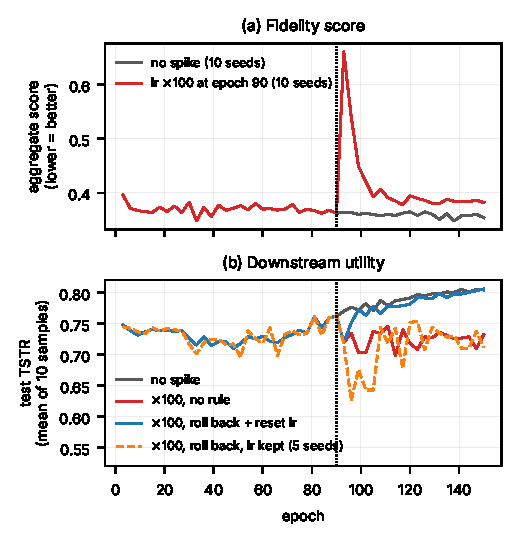
\includegraphics[width=\columnwidth]{figures/spike_rollback.pdf}
\caption{Means over seeds, learning rate \x100 at epoch 90 (dotted line).
(a) Aggregate fidelity score. (b) Test TSTR for the unspiked control, the
spiked run with no rule, roll back with the learning rate reset (10 seeds),
and roll back with the spiked learning rate kept (seeds 0--4 only). After a
rollback the final trajectory is shown.}
\label{fig:spike}
\end{figure}

\subsection{Detection with past-only references}\label{sec:detect}
Table~\ref{tab:detect} lists detected spiked runs, false alarms before the
spike, and alarms on controls. The aggregate score with an expanding
reference detected \scoreExpDet{} of 40 spiked runs with no false alarms.
By spike size, it detected \x3 in 9 of 10 runs (median delay 9 epochs),
\x10 in 10/10 (6), and \x30 and \x100 in 10/10 (3, i.e.\ the next check).
MMD$^2$ with a rolling reference detected 38 of 40.

\textbf{A detector that failed on held-out seeds.} MMD$^2$ with a fixed or
expanding reference was perfect on seeds 0--4 and was our choice before
seeing seeds 5--9. On the held-out seeds it gave false alarms on 2 of 5
controls (expanding) and 4 of 5 (fixed). In those seeds MMD$^2$ reaches its
lowest values around epochs 30--45 and then drifts up, so a reference taken
from that window is too low. A rolling reference follows the drift. We
report the aggregate score as the best detector only after looking at all 10
seeds, so its result is not a clean held-out test; a new dataset or new
seeds are needed for that.

\textbf{Threshold.} For the score (expanding), $h = 3, 4, 5, 6, 8$ gives
32/8/3, 40/0/0, 39/0/0, 38/0/0 and 32/0/0 (detected / before spike /
control alarms). Values of $h$ from 4 to 6 work; $h = 3$ is too low for every
series.

\textbf{Loss and TSTR.} The generator loss detects every spike, but whether
it raises false alarms depends on the reference: 5 of 10 controls alarm with
the expanding reference. With the fixed reference it was clean here, but it
alarmed on all 5 healthy batch-100 runs (Section~\ref{sec:start}), so we do
not consider it a reliable alarm. TSTR (mean of 10) detects only \tstrDet{}
of 40: utility is too noisy check to check to detect its own drop.

\textbf{Refitting at every check.} With the mean-shift PELT rule (seeds
0--4), results depend on the penalty, and no single penalty is best for every
series. For example, with 20 spiked runs and 5 controls, mean KS at
penalty \x1 gives 18 detected / 0 before / 0 control alarms, the aggregate
score at \x2 gives 19/0/0, and mean JSD at \x4 gives 20/0/0, but the
aggregate score and JSD at \x1 give 4 false alarms before the spike. How to
set the penalty when errors are autocorrelated is an open question.

\begin{table*}[t]
\caption{Online CUSUM detection ($k=0.5$, $h=5$). Each cell: spiked runs
detected after epoch 90 / spiked runs with an alarm before epoch 90 /
controls with an alarm. Settings were chosen on seeds 0--4. The look-ahead
rows use future checks in their reference and are shown only for
comparison.}
\label{tab:detect}
\centering
\begin{tabular}{llccc}
\toprule
Series & Reference & Seeds 0--4 (20 spiked, 5 controls) & Seeds 5--9, held out (20, 5) & All 10 seeds (40, 10) \\
\midrule
Aggregate score & expanding & 19 / 0 / 0 & 20 / 0 / 0 & 39 / 0 / 0 \\
Aggregate score & fixed & 19 / 0 / 0 & 16 / 4 / 1 & 35 / 4 / 1 \\
Aggregate score & rolling & 19 / 0 / 1 & 17 / 0 / 0 & 36 / 0 / 1 \\
MMD$^2$ & expanding & 20 / 0 / 0 & 12 / 8 / 2 & 32 / 8 / 2 \\
MMD$^2$ & fixed & 20 / 0 / 0 & 4 / 16 / 4 & 24 / 16 / 4 \\
MMD$^2$ & rolling & 19 / 0 / 0 & 19 / 0 / 0 & 38 / 0 / 0 \\
Mean KS & expanding & 15 / 0 / 0 & 18 / 0 / 0 & 33 / 0 / 0 \\
Mean JSD & expanding & 16 / 4 / 1 & 16 / 4 / 1 & 32 / 8 / 2 \\
Mean JSD & rolling & 16 / 4 / 1 & 20 / 0 / 0 & 36 / 4 / 1 \\
Correlation distance & expanding & 16 / 0 / 0 & 15 / 0 / 1 & 31 / 0 / 1 \\
Generator loss & expanding & 20 / 0 / 2 & 20 / 0 / 3 & 40 / 0 / 5 \\
Generator loss & fixed & 19 / 0 / 0 & 20 / 0 / 0 & 39 / 0 / 0 \\
TSTR (mean of 10) & expanding & 6 / 0 / 0 & 7 / 0 / 0 & 13 / 0 / 0 \\
\midrule
Aggregate score & look-ahead & 19 / 0 / 0 & 20 / 0 / 0 & 39 / 0 / 0 \\
MMD$^2$ & look-ahead & 20 / 0 / 0 & 20 / 0 / 0 & 40 / 0 / 0 \\
\bottomrule
\end{tabular}
\end{table*}

\subsection{Break or trend}
On normal runs, the rise in TSTR is a change, not a smooth trend: on 10
control runs a broken line is the best model by BIC in 8 and a mean shift in
2, and a quadratic is never best. Mean KS and mean JSD are best fit by a
straight line in 7 of 10 each, so they improve gradually; we therefore do not
claim that KS moves before TSTR. The generator loss is a bend, not a curve:
the broken line is best on all 10 controls, and the quadratic is worse by
51.7 BIC on average (33.9 to 67.1). Residual lag-1 autocorrelation is small
($-0.29$ to $0.35$ on the pilot runs), and with a long-run standard deviation
the offline CUSUM still finds a significant TSTR break in 5 of 5 pilot runs
(statistic 2.61--4.35 against a 5\% critical value of 1.358).

\subsection{Which columns the failure hits}\label{sec:percol}
Fig.~\ref{fig:percol} shows the per-column effect (seeds 0--4). The damage is
spread thinly over many columns. The largest mean effect is 4.9 noise
standard deviations (occupation at \x10). At \x100 the most affected columns
are native\_country (4.8), education (3.5) and hours\_per\_week (3.4), while
capital\_gain, capital\_loss, race and sex stay at or below 0.7 for every
spike size. At \x3 no column passes the threshold in any run, yet the
aggregate score detects most \x3 runs, because many small column changes add
up. This points to a dense change rather than a sparse one, which matters for
choosing a multivariate detector. As an offline check of a change in
\emph{which} columns are off, a cosine-kernel change detector on the
15-column vector found a change within 3 epochs of the spike in 35 of 40
spiked runs, with no change after epoch 45 on any control (penalty 0.5, chosen
on the same controls).

\begin{figure}[t]
\centering
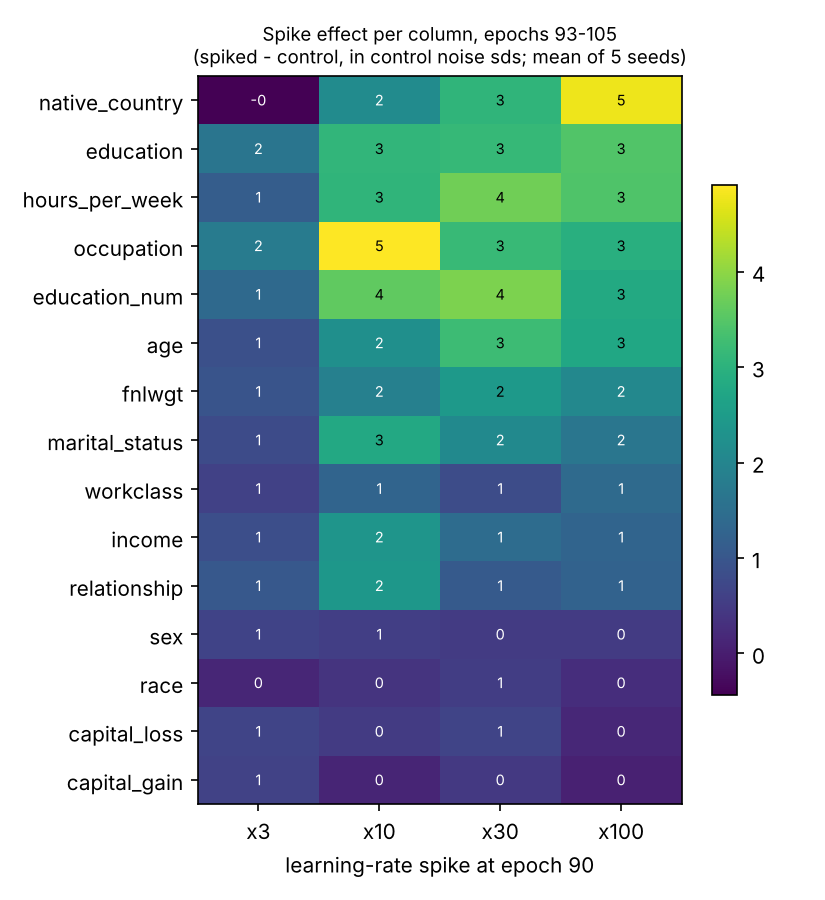
\includegraphics[width=0.85\columnwidth]{figures/per_column_effect.png}
\caption{Effect of the spike on each column, epochs 93--105: spiked minus
matched control, in units of the control's check-to-check noise (mean of
seeds 0--4).}
\label{fig:percol}
\end{figure}

\subsection{Stopping versus rolling back}
Table~\ref{tab:stop} compares stopping rules on the 50 logged runs. With a
detector that uses only past checks, ``alarm, stop and keep the onset
checkpoint'' is not reliably better than training to the end. The only gains
whose interval excludes zero are at \x100. At \x3 and \x10 even the final
spiked generator is about as good as the one before the spike, so there is
little to gain by going back. Keeping the best aggregate score is the worst
rule on spiked runs (it picks very early epochs) and also hurts on controls.
Patience on KS stops far too early. Keeping the best validation TSTR is close
to the oracle at every spike size, but needs labelled data and a known task.

\begin{table*}[t]
\caption{Test TSTR of the checkpoint each rule keeps (mean of 10 seeds). In
brackets: gain over the fixed budget $\pm$ 95\% interval half-width, in
accuracy points.}
\label{tab:stop}
\centering
\resizebox{\textwidth}{!}{%
\begin{tabular}{lccccc}
\toprule
Rule & Control & \x3 & \x10 & \x30 & \x100 \\
\midrule
Fixed budget (epoch 150) & 0.804 & 0.777 & 0.766 & 0.748 & 0.732 \\
Look-ahead CUSUM on score, keep onset & 0.804 & 0.760 ($-1.7\pm2.2$) & 0.764 ($-0.1\pm2.4$) & 0.764 ($+1.6\pm2.7$) & 0.764 ($+3.3\pm2.0$) \\
Past-only CUSUM on score (expanding), keep onset & 0.804 & 0.746 ($-3.1\pm4.6$) & 0.750 ($-1.6\pm4.7$) & 0.750 ($+0.2\pm2.3$) & 0.750 ($+1.8\pm3.9$) \\
Past-only CUSUM on MMD$^2$ (rolling), keep onset & 0.804 & 0.763 ($-1.4\pm2.2$) & 0.762 ($-0.4\pm2.5$) & 0.762 ($+1.4\pm2.6$) & 0.762 ($+3.0\pm2.1$) \\
Keep best aggregate score & 0.787 & 0.721 & 0.721 & 0.721 & 0.721 \\
Keep best mean KS & 0.795 & 0.754 & 0.744 & 0.744 & 0.744 \\
Patience 10 checks on KS & 0.733 & 0.733 & 0.733 & 0.733 & 0.733 \\
Patience 10 checks on loss & 0.730 & 0.730 & 0.730 & 0.728 & 0.721 \\
Keep best validation TSTR (labels) & 0.810 & 0.807 ($+3.0\pm1.9$) & 0.787 ($+2.1\pm1.9$) & 0.778 ($+3.0\pm1.9$) & 0.772 ($+4.1\pm2.0$) \\
Oracle (best test TSTR) & 0.811 & 0.807 & 0.787 & 0.778 & 0.773 \\
\bottomrule
\end{tabular}}
\end{table*}

\textbf{Roll back and continue.} Table~\ref{tab:rollback} shows that rolling
back and then continuing training with the learning rate reset ends at the
level of a run that never had the spike for \x10, \x30 and \x100
(\rbLow--\rbHigh{} against \dmgCtrl), better than no rule in every seed. It
also ends above keeping the best validation TSTR at \x10 to \x100 (0.787,
0.778 and 0.772), because that rule can only choose a checkpoint that
already exists. \x3 is the weak case:
one seed never alarmed, alarms came later, and the gain interval touches
zero. Every run that alarmed rolled back exactly once.

\begin{table}[t]
\caption{Roll back to the onset and keep training, learning rate reset (10
seeds). Test TSTR at the last check; differences in accuracy points, paired
by seed.}
\label{tab:rollback}
\centering
\setlength{\tabcolsep}{4pt}
\resizebox{\columnwidth}{!}{%
\begin{tabular}{lcccc}
\toprule
 & \x3 & \x10 & \x30 & \x100 \\
\midrule
Rolled back (of 10) & 9 & 10 & 10 & 10 \\
Mean alarm epoch & 101.3 & 94.8 & 93.0 & 93.3 \\
No rule & 0.777 & 0.766 & 0.748 & 0.732 \\
Roll back + continue & 0.797 & 0.805 & 0.803 & 0.805 \\
Control (no spike) & 0.804 & 0.804 & 0.804 & 0.804 \\
Rollback $-$ no rule & $+2.0\pm2.1$ & $+4.0\pm1.5$ & $+5.5\pm2.3$ & $+7.4\pm2.2$ \\
Rollback $-$ control & $-0.7\pm1.4$ & $+0.1\pm0.6$ & $-0.1\pm0.9$ & $+0.1\pm0.5$ \\
Better than no rule & 7/10 & 10/10 & 10/10 & 10/10 \\
\bottomrule
\end{tabular}}
\end{table}

\textbf{When the cause stays.} Resetting the learning rate removes the cause
we planted. If instead the spiked learning rate is kept after the restore
(Table~\ref{tab:keeplr}, seeds 0--4), every run used all 3 rollbacks within
9--18 epochs of the spike, each time restoring the same checkpoint, then
trained the rest of the run at the bad learning rate. The result is no
better than doing nothing (Fig.~\ref{fig:spike}(b), dashed). So the gain
comes from restoring \emph{and} removing the cause, not from restoring
weights alone. A usable rule would need to change something when it rolls
back, for example lower the learning rate, or stop once its rollbacks are
used up. We have not tested either.

\begin{table}[t]
\caption{Roll back with the spiked learning rate kept (seeds 0--4). Test
TSTR at the last check; differences in accuracy points.}
\label{tab:keeplr}
\centering
\resizebox{\columnwidth}{!}{%
\begin{tabular}{lcc}
\toprule
 & \x10 & \x100 \\
\midrule
No rule & 0.761 & 0.743 \\
Roll back, lr reset & 0.802 & 0.804 \\
Roll back, lr kept & 0.779 & 0.712 \\
Control & 0.804 & 0.804 \\
lr kept $-$ no rule, last check & $+1.8\pm4.3$ & $-3.2\pm6.2$ \\
lr kept $-$ no rule, mean of last 5 checks & $-0.4\pm1.9$ & $-0.6\pm1.9$ \\
\bottomrule
\end{tabular}}
\end{table}

\subsection{Problems present from the start}\label{sec:start}
Table~\ref{tab:start} compares the two changed settings with default runs of
the same seeds. A learning rate 10 times too high from the first epoch costs
about \highlrCost{} points of test TSTR and is worse in all 5 seeds, but no
detector alarms and the end-of-run fidelity metrics are no worse than a
default run's (the aggregate score is even slightly lower). There is no
change for a change detector to find: the run is worse at every check, not
from some point on. Only TSTR shows the problem. So the monitor can catch a
run that goes wrong partway through, not a run that was set up badly. Batch
size 100 turned out not to be a failure on this data (utility is the same or
slightly higher), which makes it a second kind of healthy run. On it the
score and KS detectors stay quiet, MMD$^2$ (rolling) alarms once, and the
generator loss with a fixed reference alarms on all 5 runs.

\begin{table}[t]
\caption{Settings changed from the first epoch, no spike (seeds 0--4).
Differences from default runs of the same seeds, in accuracy points.}
\label{tab:start}
\centering
\setlength{\tabcolsep}{3pt}
\resizebox{\columnwidth}{!}{%
\begin{tabular}{lccc}
\toprule
 & Default & lr \x10 from start & Batch 100 \\
\midrule
Test TSTR, last check & 0.804 & 0.761 ($-4.2\pm1.6$) & 0.807 ($+0.3\pm1.4$) \\
Test TSTR, last 5 checks & 0.803 & 0.756 ($-4.6\pm1.4$) & 0.814 ($+1.1\pm1.0$) \\
Aggregate score, last 5 & 0.355 & 0.344 & 0.352 \\
Mean KS, last 5 & 0.256 & 0.257 & 0.249 \\
Alarms: score / MMD$^2$ / KS / loss & 0/0/0/0 & 0/0/0/0 & 0/1/0/5 \\
\bottomrule
\end{tabular}}
\end{table}

\subsection{A second generator: TVAE}\label{sec:tvae}
We repeated the spike study on TVAE~\cite{xu2019ctgan} from the same
\texttt{ctgan} package (one Adam optimizer, default learning rate
$10^{-3}$, batch size 500), with the same split, checks, metrics and spike
design, on seeds 0--4 (5 controls and 20 spiked runs). TVAE has no
discriminator, so the loss series is its training loss (reconstruction plus
KL). All 20 spiked runs are identical to their controls up to epoch 90. The
detectors use the past-only settings fixed on CTGAN; nothing was tuned for
TVAE. Table~\ref{tab:tvae} gives the results.

\begin{table}[t]
\caption{TVAE, learning rate multiplied at epoch 90 (seeds 0--4). Test TSTR
at the last check; differences from the matched control in accuracy points,
paired by seed. Detection: spiked runs detected (mean delay in epochs). No
detector alarmed on a control or before the spike. One \x100 run diverged and
is excluded.}
\label{tab:tvae}
\centering
\resizebox{\columnwidth}{!}{%
\begin{tabular}{lccccc}
\toprule
 & Control & \x3 & \x10 & \x30 & \x100 \\
\midrule
Runs finished & 5 & 5 & 5 & 5 & 4 \\
Test TSTR & 0.808 & 0.802 & 0.760 & 0.767 & 0.707 \\
Spiked $-$ control & & $-0.6\pm1.5$ & $-4.8\pm2.1$ & $-4.1\pm4.1$ & $-9.8\pm11.3$ \\
Worse than control & & 3/5 & 5/5 & 4/5 & 4/4 \\
MMD$^2$, last 5 checks & 0.030 & 0.026 & 0.333 & 0.323 & 0.297 \\
\midrule
Score, expanding & 0 alarms & 0/5 & 5/5 (13.2) & 5/5 (13.8) & 4/4 (4.5) \\
MMD$^2$, rolling & 0 alarms & 3/5 (3) & 5/5 (3) & 5/5 (3) & 4/4 (3) \\
Mean KS, expanding & 0 alarms & 0/5 & 5/5 (3) & 5/5 (3) & 4/4 (3) \\
Training loss, fixed & 0 alarms & 4/5 (3) & 5/5 (3) & 5/5 (3) & 4/4 (3) \\
\bottomrule
\end{tabular}}
\end{table}

\textbf{Detection carries over.} From \x10 up the spike damages TVAE, and all
four detectors caught all 14 damaged runs that finished, with no false
alarms. MMD$^2$, mean KS and the training loss alarm at the first check after
the spike. The aggregate score, the best detector on CTGAN, is the slowest
on TVAE (about 13 epochs at \x10 and \x30).

\textbf{The damage looks different.} At \x10, TVAE's test TSTR ends at
0.755--0.766 in all 5 seeds. In seed 0 it drops from 0.820 at epoch 90 to
0.7655 at the next check and stays there; 0.7655 is the accuracy of always
predicting the majority class, so the synthetic rows no longer carry usable
information about income. Fidelity is hit much harder than for CTGAN: MMD$^2$
ends about 10 times higher than the control. At \x3, TVAE loses little
($-0.6\pm1.5$ points at the last check), while CTGAN lost about 3 points
(Table~\ref{tab:damage}). One \x100 run diverged (weights became NaN between
epochs 90 and 93), a failure that needs no detector.

\textbf{Not yet done on TVAE:} 10 seeds, stopping rules, roll back and
continue, and the break-or-trend analysis. The \x100 interval is very wide.

\subsection{Other datasets and a natural failure}
\pending{Results on two more datasets (e.g.\ a credit-default dataset and a
10,000-row subsample of Covertype) are not run yet. No failure that starts by
itself partway through a run has been found yet; the learning-rate spike is
still the only mid-run failure tested. Fill this section only from finished
runs.}

%======================================================================
\section{Discussion and Limitations}
\textbf{What the monitor is good for.} A CUSUM on an aggregate fidelity score
is cheap, needs no labels and no downstream task, and on our runs it did not
raise false alarms on normal training. It is a warning light. When labels
and a task are available, keeping the best validation-TSTR checkpoint is a
stronger selector.

\textbf{What an alarm should trigger.} Stopping and keeping the checkpoint
before the failure only recovers the generator as it was at epoch 87--90,
which is no better than what a spiked run ends with at small spike sizes.
Rolling back helps only if the cause of the failure is also removed.

\textbf{Limitations.}
(1) One dataset; CTGAN with 10 seeds, TVAE with 5 seeds and only the
damage and detection parts. (2) The only mid-run failure is a
planted learning-rate spike, which is an easy failure to detect. (3) The best
detector was picked after seeing all 10 seeds; the detector we picked in
advance failed on the held-out seeds. (4) An earlier version of our detector
used future checks in its reference; the numbers for a monitor during
training in this paper all come from past-only references. (5) In the
rollback runs, resetting the learning rate removes the planted cause, and
after a restore runs with the same seed and alarm epoch end identically, so
the 40 runs are not 40 independent outcomes; intervals are taken over seeds.
(6) BIC comparisons assume independent errors. (7) The penalty for
refitting change detection at every check is not settled. (8) The monitor
cannot see a run that is bad from the start. (9) Every fidelity metric we
tried mostly follows the time trend of training.

%======================================================================
\section{Conclusion}
On CTGAN trained on UCI Adult, a CUSUM on a simple aggregate fidelity score,
with a reference made only of past checks, detected almost every planted
mid-run failure without false alarms on normal runs, while the generator
loss and TSTR were not usable as alarms. Detecting a failure was the easier
part: stopping at the alarm did not reliably help, and rolling back helped
only when the cause of the failure was removed. The monitor cannot see a run
that was set up badly from the start. On TVAE the same detectors, with
unchanged settings, caught every damaging spike without false alarms. The
next steps are other datasets, the remaining analyses on TVAE, and a failure
that happens on its own rather than being planted.

\section*{Acknowledgment}
% CHECK WITH EACH PERSON BEFORE NAMING THEM.
\pending{Thanks to the people whose suggestions shaped the analysis; names
are added once each person has agreed to be named.}
An AI assistant (Claude, Anthropic) helped write the code and draft this
paper; this is disclosed in the repository README. Every number in the paper
comes from logged runs in the public repository.

\bibliographystyle{IEEEtran}
\bibliography{refs}

\end{document}
